\documentclass[prb,preprint]{revtex4-1} 

\usepackage{amsmath}
\usepackage{amsfonts}
\usepackage{graphicx}

\begin{document}

\title{Studying The Nature of Radiation}

\author{Ryan S. Morshead}

\affiliation{Department of Physics, California State Polytechnic University}

\date{\today}

\begin{abstract}
Using a Geiger-Mueller tube (GM-tube) to count the number of charged particles released by a sample of radium the various characteristics of its radioactivity are measured. Using the number of charged particles, or counts, over different time periods and under different conditions with the purpose of measuring background or source radiation the instrument characteristics were determined and scientific measurements were made.

After calibrating the measurement devies the source activity was calculated to be $0.139\pm0.001$ $\mu$Ci with the initial amount of atoms present in the sample being $2.589\pm0.004\times10^{13}$ atoms. Comparing the theoretical standard deviation of $31$ counts to the experimental value of $28$ counts for the high count data we find a reliability factor of $0.89$ which corresponds to at least a 90\% confidence that the data follows a Gaussian distribution. For the low count data using a Possion distribution centered around an $\bar{N}$ of 2.12 counts showed that 54\% of our counts occur between $\bar{N} \pm \sigma_{exp}$ with $\bar{N}$ being the experimental mean value and $\sigma_{exp}$ being the experimental standard deviation. This is significantly different from the ideal value of 67\%. However all of our low counts occur between $\bar{N} \pm 2\sigma_{exp}$ which corresponds closely to an ideal Poisson distribution.


\end{abstract}


\maketitle


\section{Introduction}

In 1896 the French scientist Antoine Henri Becquerel stumbled upon the phenomena of radioactivity. Using a photo sensitive plate he had intended to measure the heat radiation emitted by uranium in sunlight, however he found, after leaving the element on a photosensitive plate over night, that it had managed to activate the plate material without any outside influences\cite{henri}. Though he is recognized as the first to observe radioactivity, Becquerel never investigated the matter further. Instead he suggested that one of his students, Marie Sklodowka Curie investigate the subject for her doctoral thesis\cite{cur,henri}. So it was Curie who investigated uranium and its spontaneous emissions. During her study she quickly established that the amount of radioactivity was proportional to the amount of uranium present\cite{cur}. Additionally she found that other elements like thorium behaved similarly to uranium. With the help of her husband in 1898 she managed to demonstrate the radioactive properties of thorium and discover the highly radioactive element radium for which they earned a nobel prize\cite{cur}. Following their work Ernest Rutherford, In 1899 while studying the ionization of gases by the radiation from uranium, identified two types of ionization -- $\alpha$-radiation which produces by far the greater part of the ionization, but is absorbed by a single sheet of paper and $\beta$-radiation which produces much less ionization and is capable of penetrating several mm of dense materials like Al or Cu\cite{ernest}.

The work done in this paper seeks to explore just a few of the radioactive phenomena which were studied just prior to 1900 and that would eventually lead to the development of modern atomic theory in the early 20$^{th}$ century.

\newpage

\section{Experimental Design}

The primary measurement device responsible for collecting data directly from a radioactive source is the GM-tube. The GM-tube utilizes charged particles or photons which interact with a mica screen, to produce voltage pulses. This occurs when the cascade of electrons ionized by initial interaction with the mica screen attach to an internal, highly charged, cathode. The electrons that attach to the cathode will then create a small voltage pulse which, when amplified by a preamp, can be analyzed and enumerated by an oscilloscope or pulse counter over desired intervals. These devices, shown in Fig \ref{ExpFig}, also include a built in capacitor and resistor to reduce noise and prevent excessive current to the preamp and measuring apparatus.

\begin{figure}[h]
\centering
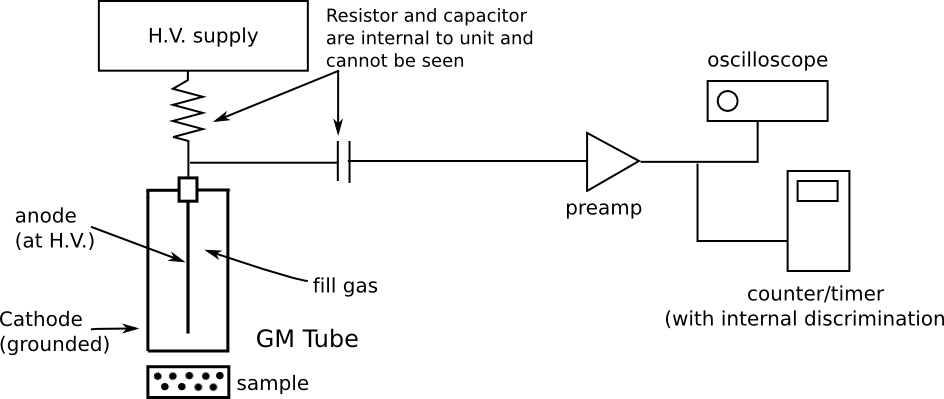
\includegraphics[scale=0.5]{GeigerMTube.png}
\caption{Gieger-Mueller tube with high voltage supply, oscilloscope, and counter}
\label{ExpFig}
\end{figure}

A number of the systems within the arrangement shown above must be calibrated to produce reliable results -- it is then necessary to characterize the GM-tube operating point, dead-time and recovery-time.

The operating point of the GM-tube, which is dependent on the magnitude of the voltage from the high voltage source, HV, as well as the characteristics of the GM-tube, is set such that ``real" or desired pulses are distinguishable from background noise. The ideal scenario is one in which the GM-tube operating point puts all desired pulses above a threshold voltage where they are thereby measurable while background pulses fall below this voltage level and are never registered. To optimize the system and approach the ideal scenario the starting point of plateau region in a counts versus HV graph should be identified -- by slowly increasing increasing the HV level from 0, the threshold voltage and thus the operating point of the GM-tube, which is only slightly less than the magnitude of the pulses being produced by the desired source, can be recognized as the point at which counts are first registered.

In this case the desired source is a sample of radium, which is an unstable nuclei that will undergo the decay 
\begin{equation}\label{eq:eq2}
_{88}Ra^{226} \rightarrow  _{86}Rn^{222}+\alpha.
\end{equation}
However because the GM-tube requires photons or particles to dislodge electrons from their host nuclei it should be noted that the $\alpha$ particle which results from this kind of decay has far too little energy to be capable of this. Thus in order to measure the number of counts the gamma rays produced by the daughter nucleus radon, which at the end of the decay is found to be in an excited state and thus, upon achieving a lower energy state, releases a photon. Then, as gamma rays from the source, or other high energy particles and photons from the background, interact with the mica window on the GM-tube, they excite electrons which are released into the gas chamber. The electrons are then accelerated by the electric field resulting from the cathode in the GM-tube. As they are accelerated the electrons collide with other electrons associated in the gas. This will either force electrons in the gas to achieve a higher potential, where upon returning to their original state they will release photons inducing further ionization, or be ionized. In either event the resulting electrons accelerate towards the cathode just as the original electron did creating an avalanche of other interactions. The cascade of ionized electrons are then collected by the cathode where they create a measurable spike of voltage. However, while the electrons are collected quickly by the cathode, the positive ions left behind by the avalanche are forced outward from the area much more slowly (on the order of milliseconds). While the ions remain collected around the cathode the electric field gradient remains too low for avalanches to propagate further and thus there is a dead time $\tau$, or period of time in which electrons released from the mica screen into the gas chamber will not be collected by the cathode. Thus there is a fraction of electrons $R_{obs} \tau$ released from the mica screen which will not produce measurable pulses, where $R_{obs}$ is the observable count rate. With this, a correction factor $C$ can be formulate to be
\begin{equation}\label{correction}
C=\frac{1}{1-R_{obs} \tau},
\end{equation}
where $CR_{obs}=R_{true}$, and $R_{true}$ is the actual count rate that would be observed absent any $\tau$. Additionally, as a consequence of the ionized plasm surrounding the cathode there is also a recovery time $t_R$ in which electrons, though having enough energy to start a cascade of interactions, will not produce interaction avalanches which are as large. Though the $t_R$ does not create a difference in the measured counts, it produces an artifact on the oscilloscope that could be misinterpreted as of the pulse width $\Delta t$ of the induced electron cascades.

Despite having the GM-tube and source material located inside a radiation barrier, there are still high energy particles and photons that manage to influence the data. As such it is important to characterize the undesired addition to the signal. Normally a Gausian distribution would be appropriate to model data with a continuous probability distribution. However, if data on the background noise is collected over short time intervals the number of counts will typically be distributed over a short range of small positive integer values, thus rendering the distribution discontinuous. In such a scenario the Possion distribution
\begin{equation}\label{eq:eq4}
P_{\mu}(\nu)=e^{-\mu} \frac{\mu^{\nu}}{\nu!},
\end{equation}
which in the limit of high $v$ values maintains a Gausian like distribution, should be used to characterize the background noise, where $\mu$ is the mean value of the distribution and $v$ is the list of positive integers ranging from 0 to $\infty$.

After removing background noise from the signal it's possible to analyze the radioactivity of the radium sample. To describe the decay of an unstable nucleus we recognize that the decay process is entirely random and that it is impossible to predict when a particular atom will decay. However, it is also equally likely for a decay to occur at any time. Therefore, given a sample of a particular radioisotope, in this case radium, the number of decay events $dN$ expected to occur in a small interval of time $dt$ is proportional to the number of atoms present $N$, that is
\begin{equation}\label{proport}
\frac{-dN}{dt}\propto N,
\end{equation}
Because one can only have a discrete number of atoms this scenario would be more accurately described by a discontinuous sum, but with an appropriately large number of initial atoms, the problem can be approximated to a partial differential equation which when solved yields
\begin{equation}\label{decay}
N=N_0e^{-t/\tau_d},
\end{equation}
where $N$ is the number of remaining nuclei after a time $t$, $N_0$ is the number of initial nuclei and $\tau_d$ is a constant given by the unique half-life of the sample $t_{1/2}$ divided by $ln(2)$.

To determined whether the least squares optimizations of the Gaussian distributions used on high count data and the Possion distribution used on the low count data are genuine approximations, a reliability factor is introduced and defined as $\sigma_{exp}/\sigma_{theo}$ where $\sigma_{e}$ is the experimental standard deviation and $\sigma_{theo}$ is the theoretical standard deviation. It is expected that if the theoretical distribution closely matches the experimental data the reliability factor should be near 1.

\newpage

\section{Data and Analysis}

To begin we identify the nature of our calibrations -- the range of voltages that make up the plateau is used to determine the percent increase of counts per 100 V. This calculation could be used to determine how linear the voltage provide by the HV was if it appeared to deviate from a linear count to voltage relationship as the average rate is related to the slope of a counts vs HV graph. Such a graph is shown in Fig. \ref{C_vs_HV}. The values $t_R$ and $\Delta t$ are also determined from an oscilloscope in order to fully describe the attributes of our calibration. Finally $\tau$ is measured from the oscilloscope and applied to Eq. \eqref{correction} in order to correct our high and low count rates.

\begin{figure}[h!]
\centering
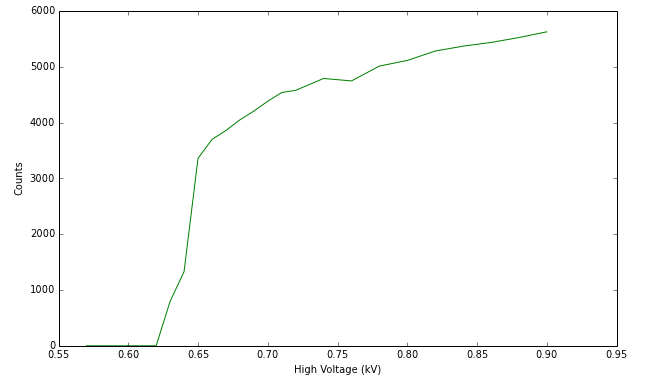
\includegraphics[scale=0.5]{C_vs_HV.png}
\caption{Counts vs HV graph of used to characterize calibration procedures with data. (note: a peak pulse voltage vs HV was also constructed but was not used to determine the plateau range)}
\label{C_vs_HV}
\end{figure}

From the data in the graph the percent increase per 100 V was determined to be $18\%\pm0.7\%$ which is near to the general approximate value of 15\% for a GM-tube. Additionally $t_R$, $\tau$, and $\Delta t$, measured at a discriminator level of 0.70 kV, were found to be $1.80\pm0.04$ ms, $0.27\pm0.02$ ms, and $60.0\pm8$ $\mu$s respectively. Based on our value for $\tau$ the count rate which would require a correction factor of 1\% would be $9.9\pm0.7\times10^{-4}$ $\mu$Ci.

With confidence that our equipment was functioning as intended we then determined the source activity of the sample in $\mu$Ci under the assumption that the half life of radium is $1602\pm0.03$ years and that the GM-tube only registers about 10\% of the decays actually undergone by a sample. The source activity was then calculated to be $0.139\pm0.001$ $\mu$Ci. Under these same assumptions the initial amount of atoms present in the sample was determined to be $2.589\times10^{13}\pm0.004$ atoms using Eq. \eqref{decay}.

After implementing the correction factor our high count data was analyzed using a least squares optimization of a Gaussian distribution shown in Fig. \ref{gauss} with a 10 count bin width histogram of the data and the fit Gaussian whose central maximum and standard deviation are approximately 99 and 31 counts respectively.

\begin{figure}[h]
\centering
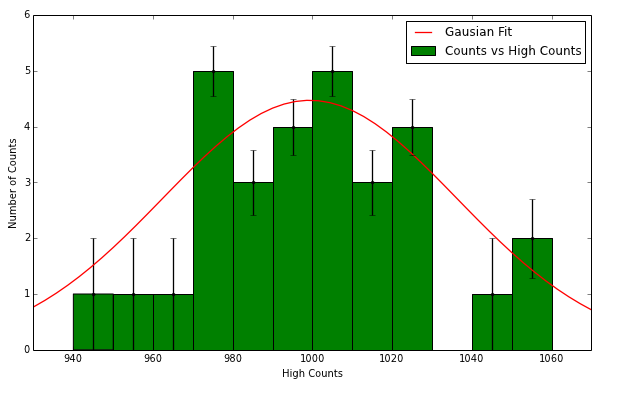
\includegraphics[scale=0.5]{C_vs_HC.png}
\caption{The corrected high count values for radium presented as a histogram with a Gaussian least squares fit}
\label{gauss}
\end{figure}

Comparing the theoretical standard deviation to the experimental value of $28$ counts yielded a reliability factor of $0.89$ which corresponds to at least a 90\% confidence that the data follows a Gaussian distribution. We also find that 63\% of the counts occur between $\bar{N} \pm \sigma_{exp}$ with $\bar{N}$ being 1001 counts, is close to the ideally Gaussian value of 68\% and that 90\% of the counts occur between $\bar{N} \pm 2\sigma_{exp}$ which is also a good approximation of the Gaussian value of 95\%. Additionally we find that the average high count rate was $10.0\pm2.8$ counts/s.

For the low count data which had an average count rate of $2.3\pm1.5$ counts/s and shown in Fig. \ref{Graph3} as a histogram with bin widths of 1 count and a Possion distribution centered around an $\bar{N}$ of 2.3 counts, we find that 80\% of our counts occur between $\bar{N} \pm \sigma_{exp}$ where $ \sigma_{exp}$ is 1.5. This is significantly different from the ideal 67\%. Additionally all of our counts occur between $\bar{N} \pm 2\sigma_{exp}$ which corresponds closely to an ideal Poisson distribution.
\begin{figure}[h]
\centering
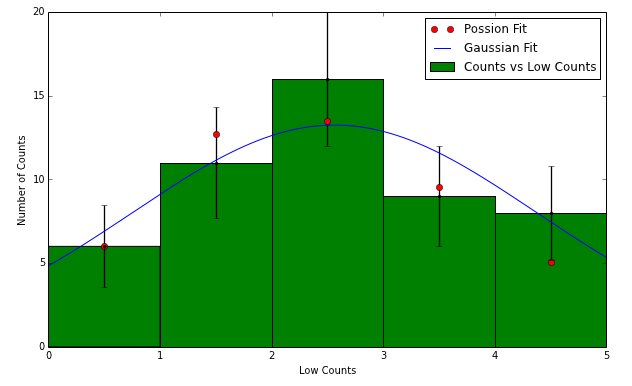
\includegraphics[scale=0.5]{C_vs_LC.png}
\caption{The corrected low count values for radium presented as a histogram with a Possion distribution centered around the experimental mean value}
\label{Graph3}
\end{figure}

\section{Conclusion}

In line with the experiments performed on radioactivity just before 1900 we found the source activity of radium to be $0.139\pm0.001$ $\mu$Ci where the initial amount of atoms present in the sample was then calculated to be$2.589\times10^{13}\pm0.004$ atoms. For high count data, comparing the theoretical standard deviation of $31$ counts to the experimental value of $28$ counts yielded a reliability factor of $0.89$ which corresponds to at least a 90\% confidence that the data follows a Gaussian distribution. For the low count data using a Possion distribution centered around an $\bar{N}$ of 2.12 counts showed that 54\% of our counts occur between $\bar{N} \pm \sigma_{exp}$. This is significantly different from the ideal value of 67\%. But we also find that all of our counts occur between $\bar{N} \pm 2\sigma_{exp}$ which corresponds closely to an ideal Poisson distribution.

\newpage

\begin{thebibliography}{99}

\bibitem{henri} Henri Becquerel (1896). ``Sur les radiations �mises par phosphorescence". Comptes Rendus \textbf{122}: 420--421.

\bibitem{cur} Mould, R. F. (1998). ``The discovery of radium in 1898 by Maria Sklodowska-Curie (1867--1934) and Pierre Curie (1859--1906) with commentary on their life and times". The British Journal of Radiology \textbf{71} (852): 1229--54.

\bibitem{ernest} Ernest Rutherford (1911). The scattering of alpha and beta particles by matter and the structure of the atom. Taylor \& Francis: 688.
\end{thebibliography}

\end{document}
